\documentclass{article}
\usepackage[a4paper,margin=1in]{geometry}
\usepackage{graphicx}
\usepackage{enumitem}
\usepackage{amsmath}
\usepackage{booktabs}
\usepackage{float}
\usepackage{xcolor}
\usepackage{tikz}
\usetikzlibrary{arrows.meta,shapes.multipart,positioning}
\usepackage{algorithm}
\usepackage{algpseudocode}
\usepackage[hidelinks]{hyperref}

% Grammar symbols and LR items
\newcommand{\tINT}{\mathtt{INT}}
\newcommand{\dt}{\mathbin{\boldsymbol{\cdot}}}
\newcommand{\Sp}{E'}
\newcommand{\la}{\quad} % separates a production from its lookaheads

% Styles shared by every automaton
\tikzset{
  lrstate/.style={draw, rounded corners=2pt, font=\scriptsize, align=left,
    inner sep=2pt, rectangle split, rectangle split parts=#1},
  lrstate/.default=2,
  lredge/.style={-{Stealth[length=2mm]}, semithick},
  lrlabel/.style={font=\scriptsize, fill=white, inner sep=1pt},
}

\title{CSE411 Assignment \#4: Bottom-Up Parsers}
\author{Sungho Kim (20241065)}
\date{\today}

\begin{document}
\maketitle

\section{Preliminaries}

\begin{table}[H]
\centering
\begin{minipage}{0.4\textwidth}
\centering
\begin{tabular}{rl}
\toprule
& Production \\
\midrule
     & $\Sp \to E\ \$$ \quad(augmented) \\
(0) & $E \to E + T$ \\
(1) & $E \to T$ \\
(2) & $T \to T * F$ \\
(3) & $T \to F$ \\
(4) & $F \to \tINT$ \\
(5) & $F \to ( E )$ \\
\bottomrule
\end{tabular}
\end{minipage}%
\begin{minipage}{0.5\textwidth}
\centering
\begin{tabular}{ccc}
\toprule
$X$ & $\mathrm{FIRST}(X)$ & $\mathrm{FOLLOW}(X)$ \\
\midrule
$E$ & $\{\tINT, (\}$ & $\{+, ), \$\}$ \\
$T$ & $\{\tINT, (\}$ & $\{+, *, ), \$\}$ \\
$F$ & $\{\tINT, (\}$ & $\{+, *, ), \$\}$ \\
\bottomrule
\end{tabular}
\end{minipage}
\caption{Numbered productions (left) and FIRST/FOLLOW sets (right).
  As in the lecture, the augmented production ends with the end marker $\$$.}
\label{tab:first-follow}
\end{table}

\noindent In every table, s$j$ means \emph{shift} the next input terminal and go to
state $j$.
r$p$ means \emph{reduce} by production $(p)$, $X \to \alpha$: pop $\alpha$ off the
stack, then go to the state given by GOTO on $X$.
acc means \emph{accept}.
Blank cells are errors.

\section{The SLR(1), LR(1), LALR(1) Parsing Tables for \textit{valid-grammar.json}}

\subsection{The SLR(1) Parsing Table for \textit{valid-grammar.json}}

\begin{table}[H]
\centering
\begin{tabular}{c cccccc ccc}
\toprule
& \multicolumn{6}{c}{ACTION} & \multicolumn{3}{c}{GOTO} \\
\cmidrule(lr){2-7}\cmidrule(lr){8-10}
State & $\tINT$ & $+$ & $*$ & $($ & $)$ & $\$$ & $E$ & $T$ & $F$ \\
\midrule
0 & s1 &  &  & s2 &  &  & 3 & 4 & 5 \\
1 &  & r4 & r4 &  & r4 & r4 &  &  &  \\
2 & s1 &  &  & s2 &  &  & 6 & 4 & 5 \\
3 &  & s7 &  &  &  & acc &  &  &  \\
4 &  & r1 & s8 &  & r1 & r1 &  &  &  \\
5 &  & r3 & r3 &  & r3 & r3 &  &  &  \\
6 &  & s7 &  &  & s9 &  &  &  &  \\
7 & s1 &  &  & s2 &  &  &  & 10 & 5 \\
8 & s1 &  &  & s2 &  &  &  &  & 11 \\
9 &  & r5 & r5 &  & r5 & r5 &  &  &  \\
10 &  & r0 & s8 &  & r0 & r0 &  &  &  \\
11 &  & r2 & r2 &  & r2 & r2 &  &  &  \\
\bottomrule
\end{tabular}
\caption{SLR(1) parsing table (12 states, conflict-free).}
\label{tab:slr}
\end{table}

\begin{figure}[H]
\centering
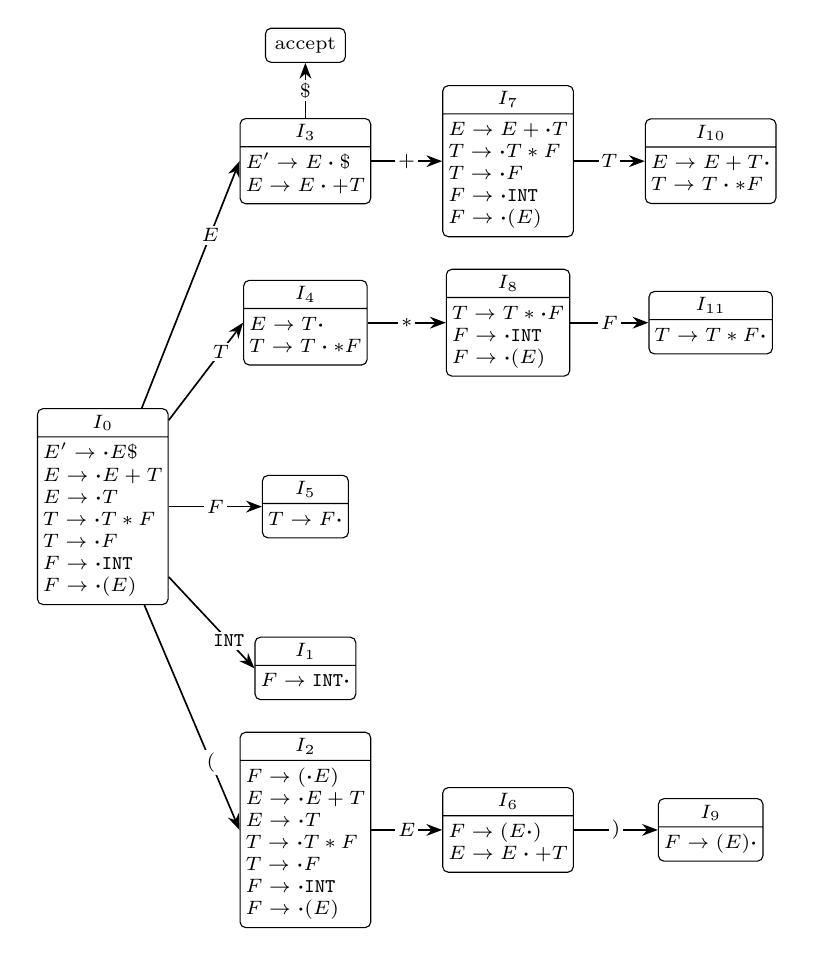
\begin{tikzpicture}
\matrix[column sep=9mm, row sep=4mm, ampersand replacement=\&] {
   \&
  \node[lrstate] (s3) {$I_{3}$ \nodepart{two} \begin{tabular}{@{}l@{}}$\Sp \to E \dt \$$ \\ $E \to E \dt + T$\end{tabular}}; \&
  \node[lrstate] (s7) {$I_{7}$ \nodepart{two} \begin{tabular}{@{}l@{}}$E \to E + \dt T$ \\ $T \to \dt T * F$ \\ $T \to \dt F$ \\ $F \to \dt \tINT$ \\ $F \to \dt ( E )$\end{tabular}}; \&
  \node[lrstate] (s10) {$I_{10}$ \nodepart{two} \begin{tabular}{@{}l@{}}$E \to E + T \dt$ \\ $T \to T \dt * F$\end{tabular}}; \\
   \&
  \node[lrstate] (s4) {$I_{4}$ \nodepart{two} \begin{tabular}{@{}l@{}}$E \to T \dt$ \\ $T \to T \dt * F$\end{tabular}}; \&
  \node[lrstate] (s8) {$I_{8}$ \nodepart{two} \begin{tabular}{@{}l@{}}$T \to T * \dt F$ \\ $F \to \dt \tINT$ \\ $F \to \dt ( E )$\end{tabular}}; \&
  \node[lrstate] (s11) {$I_{11}$ \nodepart{two} \begin{tabular}{@{}l@{}}$T \to T * F \dt$\end{tabular}}; \\
  \node[lrstate] (s0) {$I_{0}$ \nodepart{two} \begin{tabular}{@{}l@{}}$\Sp \to \dt E \$$ \\ $E \to \dt E + T$ \\ $E \to \dt T$ \\ $T \to \dt T * F$ \\ $T \to \dt F$ \\ $F \to \dt \tINT$ \\ $F \to \dt ( E )$\end{tabular}}; \&
  \node[lrstate] (s5) {$I_{5}$ \nodepart{two} \begin{tabular}{@{}l@{}}$T \to F \dt$\end{tabular}}; \&
   \&
   \\
   \&
  \node[lrstate] (s1) {$I_{1}$ \nodepart{two} \begin{tabular}{@{}l@{}}$F \to \tINT \dt$\end{tabular}}; \&
   \&
   \\
   \&
  \node[lrstate] (s2) {$I_{2}$ \nodepart{two} \begin{tabular}{@{}l@{}}$F \to ( \dt E )$ \\ $E \to \dt E + T$ \\ $E \to \dt T$ \\ $T \to \dt T * F$ \\ $T \to \dt F$ \\ $F \to \dt \tINT$ \\ $F \to \dt ( E )$\end{tabular}}; \&
  \node[lrstate] (s6) {$I_{6}$ \nodepart{two} \begin{tabular}{@{}l@{}}$F \to ( E \dt )$ \\ $E \to E \dt + T$\end{tabular}}; \&
  \node[lrstate] (s9) {$I_{9}$ \nodepart{two} \begin{tabular}{@{}l@{}}$F \to ( E ) \dt$\end{tabular}}; \\
};
\draw[lredge] (s0) -- node[lrlabel, pos=0.7] {$\tINT$} (s1.west);
\draw[lredge] (s0) -- node[lrlabel, pos=0.7] {$($} (s2.west);
\draw[lredge] (s0) -- node[lrlabel, pos=0.7] {$E$} (s3.west);
\draw[lredge] (s0) -- node[lrlabel, pos=0.7] {$T$} (s4.west);
\draw[lredge] (s0) -- node[lrlabel] {$F$} (s5);
\draw[lredge] (s2) -- node[lrlabel] {$E$} (s6);
\draw[lredge] (s3) -- node[lrlabel] {$+$} (s7);
\draw[lredge] (s4) -- node[lrlabel] {$*$} (s8);
\draw[lredge] (s6) -- node[lrlabel] {$)$} (s9);
\draw[lredge] (s7) -- node[lrlabel] {$T$} (s10);
\draw[lredge] (s8) -- node[lrlabel] {$F$} (s11);
\node[draw, rounded corners=2pt, font=\scriptsize, above=7mm of s3] (sacc) {accept};
\draw[lredge] (s3) -- node[lrlabel] {$\$$} (sacc);
\end{tikzpicture}
\caption{LR(0) automaton used by the SLR(1) table.
  Only the arrow that first reaches each state is drawn.
  The other transitions, such as $I_7 \xrightarrow{\tINT} I_1$, are the remaining
  s$j$ and GOTO entries of Table~\ref{tab:slr}.
  A completed item $X \to \alpha\dt$ (dot at the end) in $I_k$ means that $\alpha$ can
  be reduced to $X$.
  Hence, if $X \to \alpha$ is production $(p)$, row $k$ gets r$p$ for every terminal in
  $\mathrm{FOLLOW}(X)$; e.g., $F \to \tINT\dt$ in $I_1$ gives r4 on $+, *, ), \$$.}
\label{fig:lr0}
\end{figure}

\subsection{The LR(1) Parsing Table for \textit{valid-grammar.json}}

\begin{table}[H]
\centering
\begin{tabular}{c cccccc ccc}
\toprule
& \multicolumn{6}{c}{ACTION} & \multicolumn{3}{c}{GOTO} \\
\cmidrule(lr){2-7}\cmidrule(lr){8-10}
State & $\tINT$ & $+$ & $*$ & $($ & $)$ & $\$$ & $E$ & $T$ & $F$ \\
\midrule
0 & s1 &  &  & s2 &  &  & 3 & 4 & 5 \\
1 &  & r4 & r4 &  &  & r4 &  &  &  \\
2 & s6 &  &  & s7 &  &  & 8 & 9 & 10 \\
3 &  & s11 &  &  &  & acc &  &  &  \\
4 &  & r1 & s12 &  &  & r1 &  &  &  \\
5 &  & r3 & r3 &  &  & r3 &  &  &  \\
6 &  & r4 & r4 &  & r4 &  &  &  &  \\
7 & s6 &  &  & s7 &  &  & 13 & 9 & 10 \\
8 &  & s14 &  &  & s15 &  &  &  &  \\
9 &  & r1 & s16 &  & r1 &  &  &  &  \\
10 &  & r3 & r3 &  & r3 &  &  &  &  \\
11 & s1 &  &  & s2 &  &  &  & 17 & 5 \\
12 & s1 &  &  & s2 &  &  &  &  & 18 \\
13 &  & s14 &  &  & s19 &  &  &  &  \\
14 & s6 &  &  & s7 &  &  &  & 20 & 10 \\
15 &  & r5 & r5 &  &  & r5 &  &  &  \\
16 & s6 &  &  & s7 &  &  &  &  & 21 \\
17 &  & r0 & s12 &  &  & r0 &  &  &  \\
18 &  & r2 & r2 &  &  & r2 &  &  &  \\
19 &  & r5 & r5 &  & r5 &  &  &  &  \\
20 &  & r0 & s16 &  & r0 &  &  &  &  \\
21 &  & r2 & r2 &  & r2 &  &  &  &  \\
\bottomrule
\end{tabular}
\caption{Canonical LR(1) parsing table (22 states, conflict-free).}
\label{tab:lr1}
\end{table}

\begin{figure}[H]
\centering
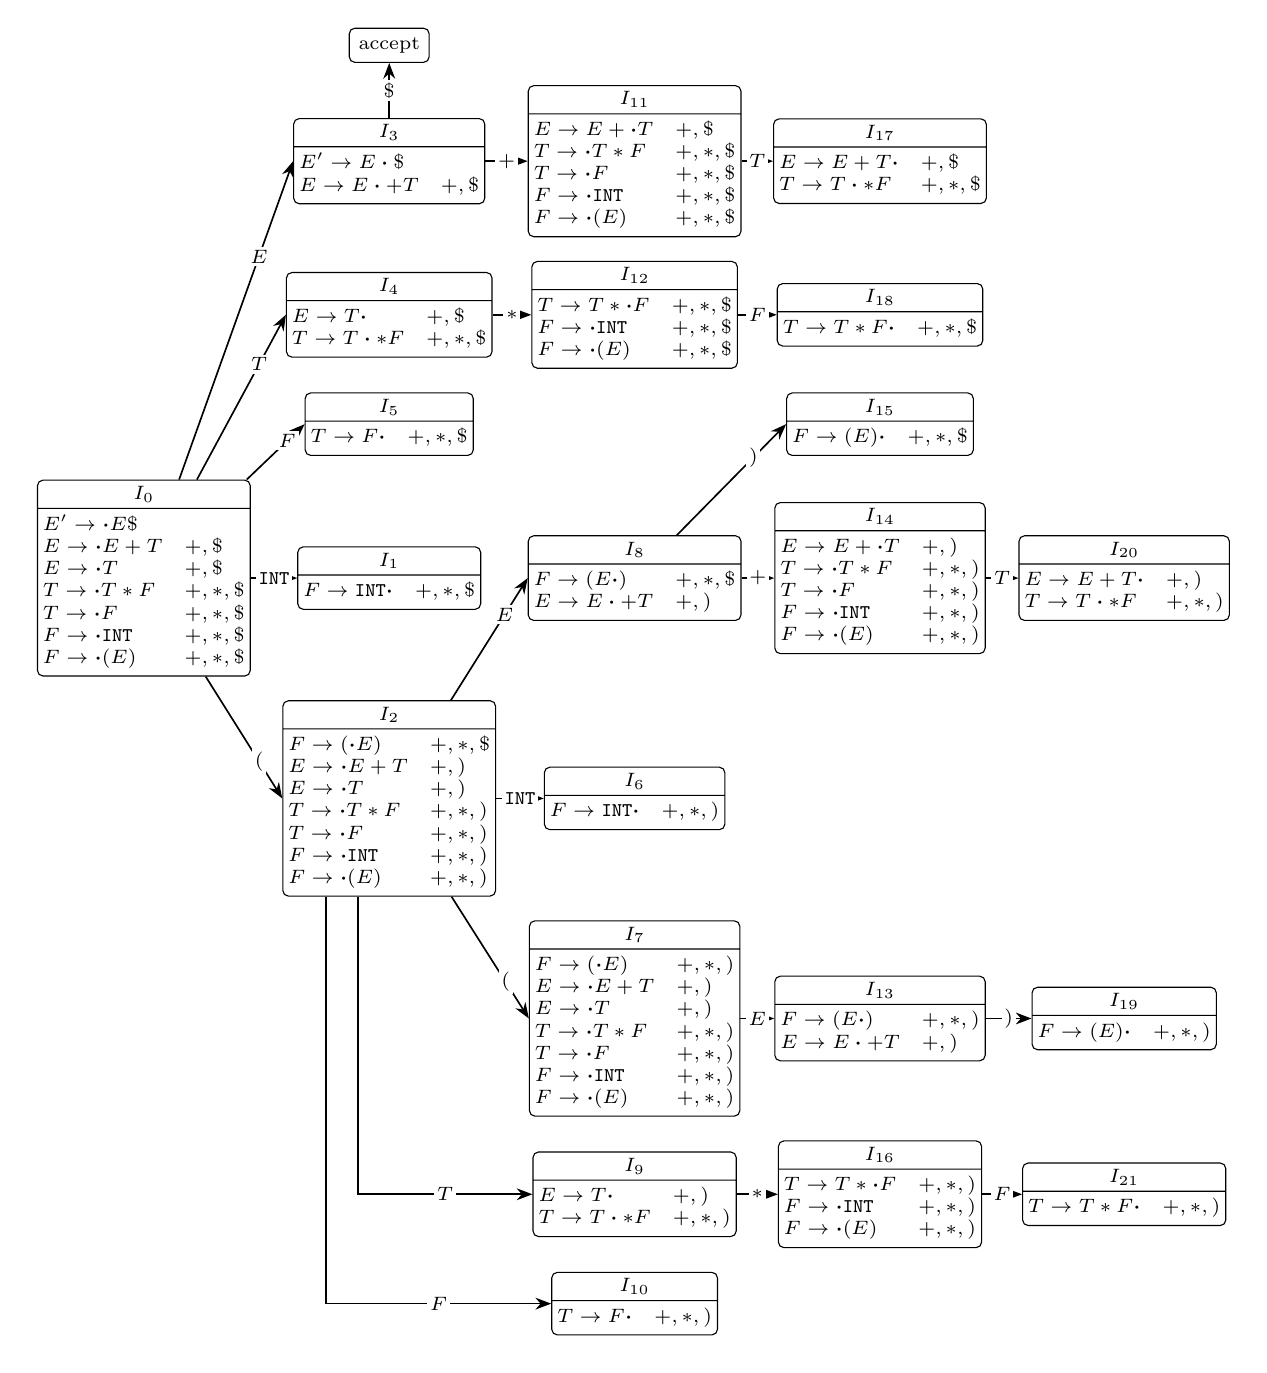
\begin{tikzpicture}
\matrix[column sep=4mm, row sep=3mm, ampersand replacement=\&] {
   \&
  \node[lrstate] (t3) {$I_{3}$ \nodepart{two} \begin{tabular}{@{}l@{\quad}l@{}}$\Sp \to E \dt \$$ &  \\ $E \to E \dt + T$ & $+, \$$\end{tabular}}; \&
  \node[lrstate] (t11) {$I_{11}$ \nodepart{two} \begin{tabular}{@{}l@{\quad}l@{}}$E \to E + \dt T$ & $+, \$$ \\ $T \to \dt T * F$ & $+, *, \$$ \\ $T \to \dt F$ & $+, *, \$$ \\ $F \to \dt \tINT$ & $+, *, \$$ \\ $F \to \dt ( E )$ & $+, *, \$$\end{tabular}}; \&
  \node[lrstate] (t17) {$I_{17}$ \nodepart{two} \begin{tabular}{@{}l@{\quad}l@{}}$E \to E + T \dt$ & $+, \$$ \\ $T \to T \dt * F$ & $+, *, \$$\end{tabular}}; \&
   \\
   \&
  \node[lrstate] (t4) {$I_{4}$ \nodepart{two} \begin{tabular}{@{}l@{\quad}l@{}}$E \to T \dt$ & $+, \$$ \\ $T \to T \dt * F$ & $+, *, \$$\end{tabular}}; \&
  \node[lrstate] (t12) {$I_{12}$ \nodepart{two} \begin{tabular}{@{}l@{\quad}l@{}}$T \to T * \dt F$ & $+, *, \$$ \\ $F \to \dt \tINT$ & $+, *, \$$ \\ $F \to \dt ( E )$ & $+, *, \$$\end{tabular}}; \&
  \node[lrstate] (t18) {$I_{18}$ \nodepart{two} \begin{tabular}{@{}l@{\quad}l@{}}$T \to T * F \dt$ & $+, *, \$$\end{tabular}}; \&
   \\
   \&
  \node[lrstate] (t5) {$I_{5}$ \nodepart{two} \begin{tabular}{@{}l@{\quad}l@{}}$T \to F \dt$ & $+, *, \$$\end{tabular}}; \&
   \&
  \node[lrstate] (t15) {$I_{15}$ \nodepart{two} \begin{tabular}{@{}l@{\quad}l@{}}$F \to ( E ) \dt$ & $+, *, \$$\end{tabular}}; \&
   \\
  \node[lrstate] (t0) {$I_{0}$ \nodepart{two} \begin{tabular}{@{}l@{\quad}l@{}}$\Sp \to \dt E \$$ &  \\ $E \to \dt E + T$ & $+, \$$ \\ $E \to \dt T$ & $+, \$$ \\ $T \to \dt T * F$ & $+, *, \$$ \\ $T \to \dt F$ & $+, *, \$$ \\ $F \to \dt \tINT$ & $+, *, \$$ \\ $F \to \dt ( E )$ & $+, *, \$$\end{tabular}}; \&
  \node[lrstate] (t1) {$I_{1}$ \nodepart{two} \begin{tabular}{@{}l@{\quad}l@{}}$F \to \tINT \dt$ & $+, *, \$$\end{tabular}}; \&
  \node[lrstate] (t8) {$I_{8}$ \nodepart{two} \begin{tabular}{@{}l@{\quad}l@{}}$F \to ( E \dt )$ & $+, *, \$$ \\ $E \to E \dt + T$ & $+, )$\end{tabular}}; \&
  \node[lrstate] (t14) {$I_{14}$ \nodepart{two} \begin{tabular}{@{}l@{\quad}l@{}}$E \to E + \dt T$ & $+, )$ \\ $T \to \dt T * F$ & $+, *, )$ \\ $T \to \dt F$ & $+, *, )$ \\ $F \to \dt \tINT$ & $+, *, )$ \\ $F \to \dt ( E )$ & $+, *, )$\end{tabular}}; \&
  \node[lrstate] (t20) {$I_{20}$ \nodepart{two} \begin{tabular}{@{}l@{\quad}l@{}}$E \to E + T \dt$ & $+, )$ \\ $T \to T \dt * F$ & $+, *, )$\end{tabular}}; \\
   \&
  \node[lrstate] (t2) {$I_{2}$ \nodepart{two} \begin{tabular}{@{}l@{\quad}l@{}}$F \to ( \dt E )$ & $+, *, \$$ \\ $E \to \dt E + T$ & $+, )$ \\ $E \to \dt T$ & $+, )$ \\ $T \to \dt T * F$ & $+, *, )$ \\ $T \to \dt F$ & $+, *, )$ \\ $F \to \dt \tINT$ & $+, *, )$ \\ $F \to \dt ( E )$ & $+, *, )$\end{tabular}}; \&
  \node[lrstate] (t6) {$I_{6}$ \nodepart{two} \begin{tabular}{@{}l@{\quad}l@{}}$F \to \tINT \dt$ & $+, *, )$\end{tabular}}; \&
   \&
   \\
   \&
   \&
  \node[lrstate] (t7) {$I_{7}$ \nodepart{two} \begin{tabular}{@{}l@{\quad}l@{}}$F \to ( \dt E )$ & $+, *, )$ \\ $E \to \dt E + T$ & $+, )$ \\ $E \to \dt T$ & $+, )$ \\ $T \to \dt T * F$ & $+, *, )$ \\ $T \to \dt F$ & $+, *, )$ \\ $F \to \dt \tINT$ & $+, *, )$ \\ $F \to \dt ( E )$ & $+, *, )$\end{tabular}}; \&
  \node[lrstate] (t13) {$I_{13}$ \nodepart{two} \begin{tabular}{@{}l@{\quad}l@{}}$F \to ( E \dt )$ & $+, *, )$ \\ $E \to E \dt + T$ & $+, )$\end{tabular}}; \&
  \node[lrstate] (t19) {$I_{19}$ \nodepart{two} \begin{tabular}{@{}l@{\quad}l@{}}$F \to ( E ) \dt$ & $+, *, )$\end{tabular}}; \\
   \&
   \&
  \node[lrstate] (t9) {$I_{9}$ \nodepart{two} \begin{tabular}{@{}l@{\quad}l@{}}$E \to T \dt$ & $+, )$ \\ $T \to T \dt * F$ & $+, *, )$\end{tabular}}; \&
  \node[lrstate] (t16) {$I_{16}$ \nodepart{two} \begin{tabular}{@{}l@{\quad}l@{}}$T \to T * \dt F$ & $+, *, )$ \\ $F \to \dt \tINT$ & $+, *, )$ \\ $F \to \dt ( E )$ & $+, *, )$\end{tabular}}; \&
  \node[lrstate] (t21) {$I_{21}$ \nodepart{two} \begin{tabular}{@{}l@{\quad}l@{}}$T \to T * F \dt$ & $+, *, )$\end{tabular}}; \\
   \&
   \&
  \node[lrstate] (t10) {$I_{10}$ \nodepart{two} \begin{tabular}{@{}l@{\quad}l@{}}$T \to F \dt$ & $+, *, )$\end{tabular}}; \&
   \&
   \\
};
\draw[lredge] (t0) -- node[lrlabel] {$\tINT$} (t1);
\draw[lredge] (t0) -- node[lrlabel, pos=0.7] {$($} (t2.west);
\draw[lredge] (t0) -- node[lrlabel, pos=0.7] {$E$} (t3.west);
\draw[lredge] (t0) -- node[lrlabel, pos=0.7] {$T$} (t4.west);
\draw[lredge] (t0) -- node[lrlabel, pos=0.7] {$F$} (t5.west);
\draw[lredge] (t2) -- node[lrlabel] {$\tINT$} (t6);
\draw[lredge] (t2) -- node[lrlabel, pos=0.7] {$($} (t7.west);
\draw[lredge] (t2) -- node[lrlabel, pos=0.7] {$E$} (t8.west);
\draw[lredge] ([xshift=-4mm]t2.south) |- node[lrlabel, pos=0.75] {$T$} (t9.west);
\draw[lredge] ([xshift=-8mm]t2.south) |- node[lrlabel, pos=0.75] {$F$} (t10.west);
\draw[lredge] (t3) -- node[lrlabel] {$+$} (t11);
\draw[lredge] (t4) -- node[lrlabel] {$*$} (t12);
\draw[lredge] (t7) -- node[lrlabel] {$E$} (t13);
\draw[lredge] (t8) -- node[lrlabel] {$+$} (t14);
\draw[lredge] (t8) -- node[lrlabel, pos=0.7] {$)$} (t15.west);
\draw[lredge] (t9) -- node[lrlabel] {$*$} (t16);
\draw[lredge] (t11) -- node[lrlabel] {$T$} (t17);
\draw[lredge] (t12) -- node[lrlabel] {$F$} (t18);
\draw[lredge] (t13) -- node[lrlabel] {$)$} (t19);
\draw[lredge] (t14) -- node[lrlabel] {$T$} (t20);
\draw[lredge] (t16) -- node[lrlabel] {$F$} (t21);
\node[draw, rounded corners=2pt, font=\scriptsize, above=7mm of t3] (tacc) {accept};
\draw[lredge] (t3) -- node[lrlabel] {$\$$} (tacc);
\end{tikzpicture}
\caption{LR(1) automaton.
  Each line is a production followed by its lookahead terminals, separated by commas;
  e.g., $F \to \tINT\dt \la +, *, \$$ in $I_1$.
  $\Sp \to \dt E\ \$$ needs no lookahead, because the $\$$ after $E$ already plays
  that role.
  The upper states (lookaheads with $\$$) belong to the outermost expression.
  The lower states (lookaheads with $)$) belong to an expression inside parentheses.
  A completed item $X \to \alpha\dt \la z_1, \dots, z_n$ in $I_k$ gives r$p$ in row $k$
  \emph{only} for $z_1, \dots, z_n$.
  As in Figure~\ref{fig:lr0}, only the arrow that first reaches each state is drawn.}
\label{fig:lr1}
\end{figure}

\subsection{The LALR(1) Parsing Table for \textit{valid-grammar.json}}

\begin{table}[H]
\centering
\begin{tabular}{c cccccc ccc}
\toprule
& \multicolumn{6}{c}{ACTION} & \multicolumn{3}{c}{GOTO} \\
\cmidrule(lr){2-7}\cmidrule(lr){8-10}
State & $\tINT$ & $+$ & $*$ & $($ & $)$ & $\$$ & $E$ & $T$ & $F$ \\
\midrule
0 & s1 &  &  & s2 &  &  & 3 & 4 & 5 \\
1 &  & r4 & r4 &  & r4 & r4 &  &  &  \\
2 & s1 &  &  & s2 &  &  & 6 & 4 & 5 \\
3 &  & s7 &  &  &  & acc &  &  &  \\
4 &  & r1 & s8 &  & r1 & r1 &  &  &  \\
5 &  & r3 & r3 &  & r3 & r3 &  &  &  \\
6 &  & s7 &  &  & s9 &  &  &  &  \\
7 & s1 &  &  & s2 &  &  &  & 10 & 5 \\
8 & s1 &  &  & s2 &  &  &  &  & 11 \\
9 &  & r5 & r5 &  & r5 & r5 &  &  &  \\
10 &  & r0 & s8 &  & r0 & r0 &  &  &  \\
11 &  & r2 & r2 &  & r2 & r2 &  &  &  \\
\bottomrule
\end{tabular}
\caption{LALR(1) parsing table (12 states, conflict-free).
  For this grammar it is identical to the SLR(1) table (Table~\ref{tab:slr}).}
\label{tab:lalr}
\end{table}

\begin{table}[H]
\centering
\setlength{\tabcolsep}{4pt}
\begin{tabular}{l *{12}{c}}
\toprule
LALR(1) state & 0 & 1 & 2 & 3 & 4 & 5 & 6 & 7 & 8 & 9 & 10 & 11 \\
\midrule
Merged LR(1) states & 0 & 1, 6 & 2, 7 & 3 & 4, 9 & 5, 10 & 8, 13 & 11, 14 & 12, 16 & 15, 19 & 17, 20 & 18, 21 \\
\bottomrule
\end{tabular}
\caption{Each LALR(1) state merges the LR(1) states (Figure~\ref{fig:lr1}) that contain
  the same items when lookaheads are ignored.}
\label{tab:merge}
\end{table}

\begin{figure}[H]
\centering
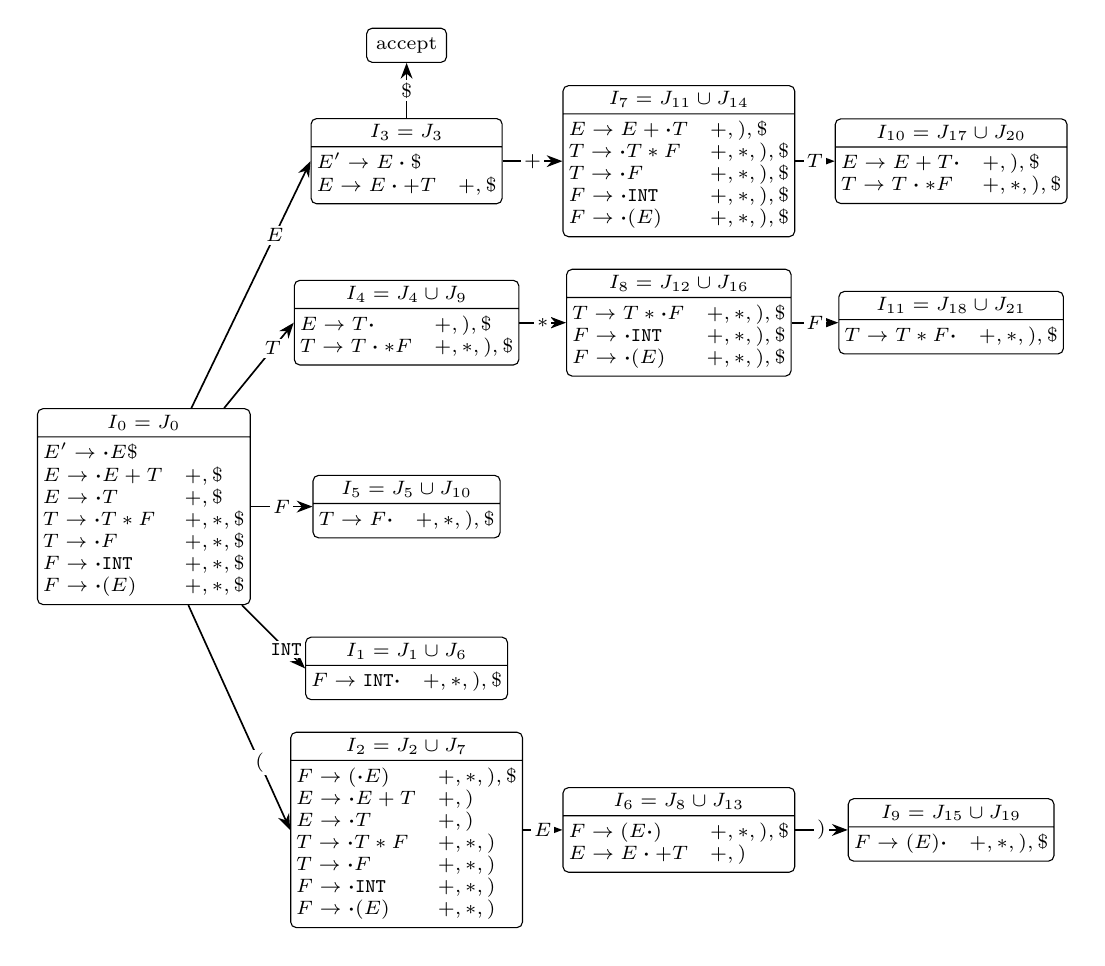
\begin{tikzpicture}
\matrix[column sep=5mm, row sep=4mm, ampersand replacement=\&] {
   \&
  \node[lrstate] (u3) {$I_{3} = J_{3}$ \nodepart{two} \begin{tabular}{@{}l@{\quad}l@{}}$\Sp \to E \dt \$$ &  \\ $E \to E \dt + T$ & $+, \$$\end{tabular}}; \&
  \node[lrstate] (u7) {$I_{7} = J_{11} \cup J_{14}$ \nodepart{two} \begin{tabular}{@{}l@{\quad}l@{}}$E \to E + \dt T$ & $+, ), \$$ \\ $T \to \dt T * F$ & $+, *, ), \$$ \\ $T \to \dt F$ & $+, *, ), \$$ \\ $F \to \dt \tINT$ & $+, *, ), \$$ \\ $F \to \dt ( E )$ & $+, *, ), \$$\end{tabular}}; \&
  \node[lrstate] (u10) {$I_{10} = J_{17} \cup J_{20}$ \nodepart{two} \begin{tabular}{@{}l@{\quad}l@{}}$E \to E + T \dt$ & $+, ), \$$ \\ $T \to T \dt * F$ & $+, *, ), \$$\end{tabular}}; \\
   \&
  \node[lrstate] (u4) {$I_{4} = J_{4} \cup J_{9}$ \nodepart{two} \begin{tabular}{@{}l@{\quad}l@{}}$E \to T \dt$ & $+, ), \$$ \\ $T \to T \dt * F$ & $+, *, ), \$$\end{tabular}}; \&
  \node[lrstate] (u8) {$I_{8} = J_{12} \cup J_{16}$ \nodepart{two} \begin{tabular}{@{}l@{\quad}l@{}}$T \to T * \dt F$ & $+, *, ), \$$ \\ $F \to \dt \tINT$ & $+, *, ), \$$ \\ $F \to \dt ( E )$ & $+, *, ), \$$\end{tabular}}; \&
  \node[lrstate] (u11) {$I_{11} = J_{18} \cup J_{21}$ \nodepart{two} \begin{tabular}{@{}l@{\quad}l@{}}$T \to T * F \dt$ & $+, *, ), \$$\end{tabular}}; \\
  \node[lrstate] (u0) {$I_{0} = J_{0}$ \nodepart{two} \begin{tabular}{@{}l@{\quad}l@{}}$\Sp \to \dt E \$$ &  \\ $E \to \dt E + T$ & $+, \$$ \\ $E \to \dt T$ & $+, \$$ \\ $T \to \dt T * F$ & $+, *, \$$ \\ $T \to \dt F$ & $+, *, \$$ \\ $F \to \dt \tINT$ & $+, *, \$$ \\ $F \to \dt ( E )$ & $+, *, \$$\end{tabular}}; \&
  \node[lrstate] (u5) {$I_{5} = J_{5} \cup J_{10}$ \nodepart{two} \begin{tabular}{@{}l@{\quad}l@{}}$T \to F \dt$ & $+, *, ), \$$\end{tabular}}; \&
   \&
   \\
   \&
  \node[lrstate] (u1) {$I_{1} = J_{1} \cup J_{6}$ \nodepart{two} \begin{tabular}{@{}l@{\quad}l@{}}$F \to \tINT \dt$ & $+, *, ), \$$\end{tabular}}; \&
   \&
   \\
   \&
  \node[lrstate] (u2) {$I_{2} = J_{2} \cup J_{7}$ \nodepart{two} \begin{tabular}{@{}l@{\quad}l@{}}$F \to ( \dt E )$ & $+, *, ), \$$ \\ $E \to \dt E + T$ & $+, )$ \\ $E \to \dt T$ & $+, )$ \\ $T \to \dt T * F$ & $+, *, )$ \\ $T \to \dt F$ & $+, *, )$ \\ $F \to \dt \tINT$ & $+, *, )$ \\ $F \to \dt ( E )$ & $+, *, )$\end{tabular}}; \&
  \node[lrstate] (u6) {$I_{6} = J_{8} \cup J_{13}$ \nodepart{two} \begin{tabular}{@{}l@{\quad}l@{}}$F \to ( E \dt )$ & $+, *, ), \$$ \\ $E \to E \dt + T$ & $+, )$\end{tabular}}; \&
  \node[lrstate] (u9) {$I_{9} = J_{15} \cup J_{19}$ \nodepart{two} \begin{tabular}{@{}l@{\quad}l@{}}$F \to ( E ) \dt$ & $+, *, ), \$$\end{tabular}}; \\
};
\draw[lredge] (u0) -- node[lrlabel, pos=0.7] {$\tINT$} (u1.west);
\draw[lredge] (u0) -- node[lrlabel, pos=0.7] {$($} (u2.west);
\draw[lredge] (u0) -- node[lrlabel, pos=0.7] {$E$} (u3.west);
\draw[lredge] (u0) -- node[lrlabel, pos=0.7] {$T$} (u4.west);
\draw[lredge] (u0) -- node[lrlabel] {$F$} (u5);
\draw[lredge] (u2) -- node[lrlabel] {$E$} (u6);
\draw[lredge] (u3) -- node[lrlabel] {$+$} (u7);
\draw[lredge] (u4) -- node[lrlabel] {$*$} (u8);
\draw[lredge] (u6) -- node[lrlabel] {$)$} (u9);
\draw[lredge] (u7) -- node[lrlabel] {$T$} (u10);
\draw[lredge] (u8) -- node[lrlabel] {$F$} (u11);
\node[draw, rounded corners=2pt, font=\scriptsize, above=7mm of u3] (uacc) {accept};
\draw[lredge] (u3) -- node[lrlabel] {$\$$} (uacc);
\end{tikzpicture}
\caption{LALR(1) automaton. $J_k$ is state $k$ of the LR(1) automaton
  (Figure~\ref{fig:lr1}), and each lookahead list is the union over the merged states.
  Without the lookaheads, the states and arrows are exactly those of the LR(0) automaton
  (Figure~\ref{fig:lr0}).}
\label{fig:lalr}
\end{figure}

\section{Parsing Table Construction}

Each construction builds an automaton of item sets, then uses its transitions and
completed items to fill the parsing table.
An edge $I_k \xrightarrow{Y} I_j$ gives s$j$ in ACTION$[k, Y]$ if $Y$ is a terminal,
and $j$ in GOTO$[k, Y]$ if $Y$ is a nonterminal.
The edge $I_3 \xrightarrow{\$} \text{accept}$ gives acc.
States are numbered in the order they are added: the implementation scans the states
in that order and tries the symbols in the order $\tINT, +, *, (, ), E, T, F$.
The methods use different state sets and reduction lookaheads.
A cell with two actions would be a conflict.
None of the three tables has one, so the grammar is SLR(1), LR(1), and LALR(1).

\subsection{SLR(1) Construction}

\begin{enumerate}[leftmargin=*]
  \item Compute FIRST and FOLLOW (Table~\ref{tab:first-follow}, Algorithm~\ref{alg:first-follow}).
  \item Build the LR(0) automaton (Figure~\ref{fig:lr0}) with Algorithm~\ref{alg:lr0},
    starting from $\textsc{Closure}(\{\Sp \to \dt E\ \$\})$.
    This yields 12 states.
  \item Fill the table (Algorithm~\ref{alg:slr-table}).
    A completed item $X \to \alpha\dt$ in $I_k$ puts r$p$ in every column
    $a \in \mathrm{FOLLOW}(X)$.
    For example, $I_1 = \{F \to \tINT\dt\}$ reduces by (4) on
    $\mathrm{FOLLOW}(F) = \{+, *, ), \$\}$.
    $I_4$ contains both $E \to T\dt$ and $T \to T\dt * F$, so it reduces by (1) on
    $\mathrm{FOLLOW}(E) = \{+, ), \$\}$ and shifts on $*$.
    Since $* \notin \mathrm{FOLLOW}(E)$, there is no shift/reduce conflict.
    The same applies to $I_{10}$.
\end{enumerate}

\subsection{LR(1) Construction}

\begin{enumerate}[leftmargin=*]
  \item Each item now carries a lookahead $z$: a terminal that can come next once the
    item is completed.
    For an item $X \to \alpha \dt Y \beta \la z$, \textsc{Closure} gives each new item
    $Y \to \dt \gamma$ the lookaheads $\mathrm{FIRST}(\beta z)$
    (Algorithm~\ref{alg:lr1}).
    For example, in $I_2$ the items for $E$ get $+, )$, because $E$ is followed by $)$
    in $F \to ( \dt E )$ and by $+$ in $E \to \dt E + T$.
  \item Run the main loop of Algorithm~\ref{alg:lr0} with this \textsc{Closure} and
    \textsc{Goto}.
    Two states are equal only if their items \emph{and} lookaheads match.
    So every LR(0) state that can be reached both outside parentheses (followed by $\$$)
    and inside them (followed by $)$) splits in two.
    Examples are $I_1$ and $I_6$ (both $F \to \tINT\dt$), and $I_5$ and $I_{10}$.
    Only the states with $\Sp$ items ($I_0$ and $I_3$) occur solely at the top level.
    The other 10 LR(0) states appear twice, so there are $12 + 10 = 22$ states.
  \item Fill the table (Algorithm~\ref{alg:lr1-table}).
    A completed item $X \to \alpha\dt \la z_1, \dots, z_n$ reduces \emph{only} on
    $z_1, \dots, z_n$.
    Hence row 1 reduces on $+, *, \$$ but not on $)$, and row 6 reduces on $+, *, )$
    but not on $\$$.
    The SLR table instead reduces on all of $\mathrm{FOLLOW}(F)$.
    For example, after reading a top-level $\tINT$ with $)$ next in the input,
    LR(1) reports an error in state 1; SLR(1) first reduces by (4).
\end{enumerate}

\subsection{LALR(1) Construction}

\begin{enumerate}[leftmargin=*]
  \item Build the LR(1) automaton.
    Then merge all states that contain the same items when lookaheads are ignored,
    taking the union of their lookaheads (Algorithm~\ref{alg:lalr}).
    Merged states are numbered in the order in which their first LR(1) state appears.
    Table~\ref{tab:merge} lists the 12 merged groups.
  \item Merged states have transitions on the same symbols, and those transitions
    lead to states that are merged together as well.
    So the merged automaton is still deterministic.
    Without lookaheads it is the LR(0) automaton, with the same numbering here
    (Figure~\ref{fig:lalr}).
  \item Fill the table exactly as for LR(1), using the merged lookaheads
    (Algorithm~\ref{alg:lr1-table}).
    Merging can create reduce/reduce conflicts but never new shift/reduce conflicts.
    No conflicts occur for this grammar.
    For every completed item here, the merged lookaheads equal the FOLLOW set of its left-hand side;
    for example, $I_4$ has $E \to T\dt \la +, ), \$$, and
    $\mathrm{FOLLOW}(E) = \{+, ), \$\}$.
    So the LALR(1) table coincides with the SLR(1) table.
\end{enumerate}

\clearpage
\section*{Appendices}
\addcontentsline{toc}{section}{Appendices}
\setcounter{subsection}{0}
\renewcommand{\thesubsection}{Appendix \Alph{subsection}}
\makeatletter
\@addtoreset{algorithm}{subsection}
\makeatother
\renewcommand{\thealgorithm}{\Alph{subsection}.\arabic{algorithm}}

\subsection{SLR(1) Construction}

Algorithm~\ref{alg:first-follow} computes FIRST and FOLLOW until the sets stop
changing.
$\mathrm{FIRST}(Y_1 \cdots Y_n)$ is $\mathrm{FIRST}(Y_1)$ without $\varepsilon$, plus
$\mathrm{FIRST}(Y_2 \cdots Y_n)$ if $Y_1$ can derive $\varepsilon$; the empty string has
$\mathrm{FIRST} = \{\varepsilon\}$.
Algorithm~\ref{alg:lr0} is the LR(0) automaton construction of the lecture
(\textit{LR.html}, slide~23).
Algorithm~\ref{alg:slr-table} fills the SLR(1) table from that automaton.

\begin{algorithm}[H]
\caption{FIRST and FOLLOW sets}
\label{alg:first-follow}
\begin{algorithmic}[1]
\State $\mathrm{FIRST}(a) \gets \{a\}$ for each terminal $a$;\quad $\mathrm{FIRST}(X) \gets \emptyset$ for each nonterminal $X$
\Repeat
  \ForAll{productions $X \to Y_1 \cdots Y_n$}
    \State add $\mathrm{FIRST}(Y_1 \cdots Y_n)$ to $\mathrm{FIRST}(X)$
  \EndFor
\Until{no FIRST set changes}
\State $\mathrm{FOLLOW}(X) \gets \emptyset$ for each nonterminal $X$ \Comment{$\Sp \to E\ \$$ puts $\$$ in $\mathrm{FOLLOW}(E)$}
\Repeat
  \ForAll{productions $X \to \alpha Y \beta$ with $Y$ a nonterminal}
    \State add $\mathrm{FIRST}(\beta) \setminus \{\varepsilon\}$ to $\mathrm{FOLLOW}(Y)$
    \If{$\varepsilon \in \mathrm{FIRST}(\beta)$} add $\mathrm{FOLLOW}(X)$ to $\mathrm{FOLLOW}(Y)$ \EndIf
  \EndFor
\Until{no FOLLOW set changes}
\end{algorithmic}
\end{algorithm}

\begin{algorithm}[H]
\caption{LR(0) automaton construction (lecture slide 23)}
\label{alg:lr0}
\begin{algorithmic}[1]
\State $CS \gets \emptyset$ \Comment{a set of closures}
\State $CS \gets CS \cup \{\textsc{Closure}(\{\Sp \to \dt E\ \$\})\}$ \Comment{$E$ is the start nonterminal}
\State $\mathit{Edges} \gets \emptyset$
\Repeat
  \ForAll{$C \in CS$}
    \ForAll{items $X \to \alpha \dt Y \beta$ in $C$} \Comment{$Y$ is a terminal or a nonterminal}
      \If{$Y$ is not $\$$}
        \State let $J$ be $\textsc{Goto}(C, Y)$
        \State $CS \gets CS \cup \{J\}$
        \State $\mathit{Edges} \gets \mathit{Edges} \cup \{C \xrightarrow{Y} J\}$
      \Else
        \State $\mathit{Edges} \gets \mathit{Edges} \cup \{C \xrightarrow{\$} \text{accept}\}$
      \EndIf
    \EndFor
  \EndFor
\Until{$CS$ and $\mathit{Edges}$ do not change}
\Statex
\Function{Closure}{$I$}
  \Repeat
    \ForAll{items $X \to \alpha \dt Y \beta$ in $I$}
      \ForAll{productions $Y \to \gamma$}
        \State $I \gets I \cup \{Y \to \dt \gamma\}$
      \EndFor
    \EndFor
  \Until{$I$ does not change}
  \State \Return $I$
\EndFunction
\Statex
\Function{Goto}{$I, Y$}
  \State $J \gets \emptyset$
  \ForAll{items $X \to \alpha \dt Y \beta$ in $I$}
    \State $J \gets J \cup \{X \to \alpha Y \dt \beta\}$
  \EndFor
  \State \Return $\textsc{Closure}(J)$
\EndFunction
\end{algorithmic}
\end{algorithm}

\begin{algorithm}[H]
\caption{SLR(1) table construction}
\label{alg:slr-table}
\begin{algorithmic}[1]
\Require LR(0) automaton $(CS, \mathit{Edges})$ with states $I_0, I_1, \dots$
\ForAll{edges $I_k \xrightarrow{Y} I_j$ in $\mathit{Edges}$}
  \If{$Y$ is a terminal} add s$j$ to ACTION$[k, Y]$
  \Else\ GOTO$[k, Y] \gets j$
  \EndIf
\EndFor
\ForAll{edges $I_k \xrightarrow{\$} \text{accept}$ in $\mathit{Edges}$} add acc to ACTION$[k, \$]$ \EndFor
\ForAll{states $I_k$ and completed items $X \to \alpha \dt$ in $I_k$}
  \State let $(p)$ be the number of production $X \to \alpha$
  \ForAll{$a \in \mathrm{FOLLOW}(X)$} add r$p$ to ACTION$[k, a]$ \EndFor
\EndFor
\State report every ACTION cell with more than one action as a conflict
\end{algorithmic}
\end{algorithm}

\subsection{LR(1) Construction}

Algorithm~\ref{alg:lr1} is the LR(1) automaton construction of the lecture
(slide~24).
Its main loop is that of Algorithm~\ref{alg:lr0}; only \textsc{Closure} and \textsc{Goto}
change, so that every item $(X \to \alpha \dt \beta, z)$ carries a lookahead terminal $z$.
Algorithm~\ref{alg:lr1-table} fills the table, reducing only on each item's own
lookahead.

\begin{algorithm}[H]
\caption{LR(1) automaton construction (lecture slide 24)}
\label{alg:lr1}
\begin{algorithmic}[1]
\State run lines 1--16 of Algorithm~\ref{alg:lr0} with the \textsc{Closure} and \textsc{Goto} below
\Statex \Comment{$\Sp \to \dt E\ \$$ needs no lookahead: $\mathrm{FIRST}(\$\, z) = \{\$\}$ for every $z$}
\Statex
\Function{Closure}{$I$}
  \Repeat \Comment{$z$: lookahead terminal}
    \ForAll{items $(X \to \alpha \dt Y \beta, z)$ in $I$}
      \ForAll{productions $Y \to \gamma$} \Comment{$Y$ is a nonterminal}
        \ForAll{$w \in \mathrm{FIRST}(\beta z)$}
          \State $I \gets I \cup \{(Y \to \dt \gamma, w)\}$
        \EndFor
      \EndFor
    \EndFor
  \Until{$I$ does not change}
  \State \Return $I$
\EndFunction
\Statex
\Function{Goto}{$I, Y$}
  \State $J \gets \emptyset$
  \ForAll{items $(X \to \alpha \dt Y \beta, z)$ in $I$}
    \State $J \gets J \cup \{(X \to \alpha Y \dt \beta, z)\}$ \Comment{the lookahead is kept}
  \EndFor
  \State \Return $\textsc{Closure}(J)$
\EndFunction
\end{algorithmic}
\end{algorithm}

\begin{algorithm}[H]
\caption{LR(1) table construction (also used for LALR(1))}
\label{alg:lr1-table}
\begin{algorithmic}[1]
\Require LR(1) automaton $(CS, \mathit{Edges})$ with states $I_0, I_1, \dots$
\State fill the s$j$, GOTO, and acc entries as in lines 1--7 of Algorithm~\ref{alg:slr-table}
\ForAll{states $I_k$ and completed items $(X \to \alpha \dt, z)$ in $I_k$}
  \State let $(p)$ be the number of production $X \to \alpha$
  \State add r$p$ to ACTION$[k, z]$ \Comment{only the item's own lookahead}
\EndFor
\State report every ACTION cell with more than one action as a conflict
\end{algorithmic}
\end{algorithm}

\subsection{LALR(1) Construction}

Algorithm~\ref{alg:lalr} merges the LR(1) states that contain the same items once
lookaheads are ignored ($\mathrm{strip}$ below).
Lines 2--8 merge the states, and line 9 redirects every edge to the merged states.
The result is still deterministic: merged states have transitions on the same symbols,
and those transitions lead to states that are merged together as well.
The table is then filled by Algorithm~\ref{alg:lr1-table}.

\begin{algorithm}[H]
\caption{LALR(1) by merging LR(1) states}
\label{alg:lalr}
\begin{algorithmic}[1]
\Require LR(1) automaton with states $J_0, \dots, J_{n-1}$ and $\mathit{Edges}$;\quad $\mathrm{strip}(J) = \{X \to \alpha \dt \beta \mid (X \to \alpha \dt \beta, z) \in J\}$
\State $m \gets 0$ \Comment{number of LALR(1) states so far}
\For{$k \gets 0$ \textbf{to} $n - 1$} \Comment{in LR(1) state order}
  \If{$\mathrm{strip}(J_k) = \mathrm{strip}(I_i)$ for some $i < m$}
    \State $I_i \gets I_i \cup J_k$;\quad $\mathit{num}(k) \gets i$ \Comment{union of lookaheads}
  \Else
    \State $I_m \gets J_k$;\quad $\mathit{num}(k) \gets m$;\quad $m \gets m + 1$
  \EndIf
\EndFor
\State $\mathit{Edges}' \gets \{I_{\mathit{num}(k)} \xrightarrow{Y} I_{\mathit{num}(j)} \mid J_k \xrightarrow{Y} J_j \in \mathit{Edges}\} \cup \{I_{\mathit{num}(k)} \xrightarrow{\$} \text{accept} \mid J_k \xrightarrow{\$} \text{accept} \in \mathit{Edges}\}$
\State \Return states $I_0, \dots, I_{m-1}$ and $\mathit{Edges}'$
\end{algorithmic}
\end{algorithm}

\end{document}
